\documentclass[conference]{IEEEtran}

\renewcommand{\familydefault}{\sfdefault}

\usepackage{graphicx}
\usepackage{caption}
\usepackage{subfigure}
\usepackage{float}
\usepackage{indentfirst}
\usepackage[compact]{titlesec}
\setlength{\parindent}{11pt}
\newcommand{\forceindent}{\leavevmode{\parindent=1em\indent}}

\hyphenation{op-tical net-works semi-conduc-tor}

\graphicspath{{images/}}

\usepackage{hyperref}

\hypersetup
{
    colorlinks=true,
    linkcolor=black,   
    urlcolor=blue,
    citecolor=black,
}


\begin{document}



\title{AINT308 - OpenCV Assignment 1 2022}

\author{\IEEEauthorblockN{Student No. 10618407}
\IEEEauthorblockA{School of Engineering,\\Computing and Mathematics
\\University of Plymouth\\
Plymouth, Devon\\}}

\maketitle

\begin{abstract}

Machine vision is a mature technology that is becoming more prevalent within modern engineering practises. It is being utilised more in the rapidly evolving fields of autonomy and automation. This report outlines some of the functionalities of a popular C/C++ based computer visions library \href{https://opencv.org}{\textit{OpenCV}}. The Assignment has been split into three tasks; Task 1, Task 2, and Task 3. The first task, Task 1, is to evaluate the colors of pixels in a picture to determine the colour of a given object in the frame (car). The second task, Task 2, was to track on object across multiple frames of a video to track its motion (swinging pendulum). The final task, Task 3, was to identify and cross correlate components on a circuit to check for any missing components.

\end{abstract}

\subsection*{Keywords:} 
Computer Vision, OpenCV, Object Detection, C++, Object Tracking

\section{Task 1: Colour Sorter}	
\subsection{Introduction}
The first task was to evaluate the colour of a given object within a frame color within the RGB colour space. For this task, the colour of the car within a frame is being evaluated. An example of the type of image can be seen in Fig. \ref{fig:example_car}.

\begin{figure}
\centerline{\includegraphics[width=.4\textwidth]{example_car}}
\caption{Example Car Image}
\label{fig:example_car}
\end{figure}

\subsection{Solution}
Fig. \ref{fig:CW1_Task_1_code_colour_checker} shows the solution to the first task, the Colour Sorter.

\begin{figure}{H}
\centerline{\includegraphics[width=.5\textwidth]{CW1_Task_1_code_colour_checker}}
\caption{Task 1 Code - Colour Checking}
\label{fig:CW1_Task_1_code_colour_checker}
\end{figure}

\textbf{OpenCV} includes a built in method for retrieving the values of a pixel in an image. The code begins by iterating through two loops, one to look at all the rows and the second to go through all the columns. If one of the R(red), G(green), or B(blue) value is more than $1.5$ times larger than the others the pixel is deemed to be that colour. This is done to help distinguish between the vibrant colour of the car and what could be considered the background in the image. Once this pixel has been checked, if the colour is within the given threshold, it is added to a running total for each of the colours.

The value of $1.5$ was chosen because it was deemed to be a significant enough proportion larger that it was definitive in selecting the colour. If the value was too high, none of the colours would ever have been selected. If the value was too low, it would potentially get confused between the RGB values, especially for colours with a similar spread.

After the whole image is checked, the counts are totalled and the highest value is deemed to be the colour of the car. This can be seen in Fig. \ref{fig:CW1_Task_1_code_colour_checker_output}.

A flow chart for this task can be seen in Appendix \ref{appendix:task_1_flowchart}.

\begin{figure}
\centerline{\includegraphics[width=.5\textwidth]{CW1_Task_1_code_colour_checker_output}}
\caption{Task 1 Code - Output}
\label{fig:CW1_Task_1_code_colour_checker_output}
\end{figure}

To test the algorithm further, a larger dataset of pictures of cars was used. 40 more images of cars were added to the dataset, alongside the original 30 that was provided. The new dataset was initially used to train and test machine learning models. \cite{ref:KrauseStarkDengFei-Fei_3DRR2013} These were added to test how to algorithms functionality was maintained up without the use of highly cropped and optimised inputs.

Overall this method worked for the dataset that was provided this can be seen in Table \ref{table:car_colours_original_dataset}.

\begin{table}
\begin{center}
\caption{Number of Correct Car Colour Calculations - original dataset}
\begin{tabular}{ || c || c || c || }
\hline
 Red & Blue & Green\\ 
\hline
 10/10 & 10/10 & 10/10 \\  
\hline

\end{tabular}
\label{table:car_colours_original_dataset}
\end{center}
\end{table}

It can be seen in Table \ref{table:car_colours_expanded_dataset} that using non-sanitised inputs. The colour sorter does not perform as well. The only colour of car that was correctly identified consistently was red.  There were some other colours not accounted for by the colour sorter. The output RGB values for the colours did not appear to represent these colours. This was only done out of interest and gave no meaningful data to analyse. 

\begin{table}
\begin{center}
\caption{Number of Correct Car Colour Calculations - expanded dataset}
\begin{tabular}{ || c || c || c || c || c || c || c || }
\hline
 Red & Blue & Green & Black & Silver & Yellow & White\\ 
\hline
 13/13 & 11/12 & 2/7 & 0/1 & 0/4 & 0/2 & 0/1 \\  
\hline

\end{tabular}
\label{table:car_colours_expanded_dataset}
\end{center}
\end{table}


The original dataset was selected such that the car made up a majority of the frame and the background was for the most part plain, as to not sway the results.

\textit{A video of the code in operation can be seen in this \href{https://youtu.be/hWfO3ubkQVc}{link}}


\subsection{Further Improvements}
Although this task worked for the given dataset, there are ways to improve the colour detection accuracy. RGB models are typically not used for this type of task, with the Hue, Saturation, and Value (HSV) model being preferred. Initially the RGB model was built and optimised to be used on display screens, whereas the HSV model was developed to mimic how a human interpret colours. Since HSV models are able to separate colour values, saturation, and lightness, operations can be more easily performed on the hue itself. Because we are more interested in the colour of the cars and not the lightness, a HSV colour model would be an objectively better solution. \cite{ref:HSV_vs_RGB}

Another improvement is to make the algorithm detect the outline of the car. This would eliminate the issues caused by having a background that could be mistaken for the body of the car. An example of this can be seen in Fig \ref{fig:red_car_green_background}. Open CV is capable of detecting cars in images and videos, albeit trivially. Although trivial, it could be used to draw a box around the car thus eliminating the background surrounding the car. \cite{ref:Vehicle_detection_in_python} 

\begin{figure}
\centerline{\includegraphics[width=.5\textwidth]{red_car_green_background}}
\caption{Example Car with undesirable background}
\label{fig:red_car_green_background}
\end{figure}

The red car with a green background may confuse the simple sorting algorithm and lead to a false result (the algorithm may think the car is green). This is the issue with using such a basic classification algorithm.

The final improvement that could be partially solved by using the HSV colour model, but that would also require a far more complex solving algorithm \cite{ref:colour_sorting}, is that cars are not just red, green, or blue. They come in many different colours (including white, black, and silver) and also in many different shades and brightness of colour. By isolating just the RGB values and evaluating which is highest, a lot of granularity is lost. Using this method it is impossible to detect the shade of the car and even the type of red, green, or blue the car may be, if it is one of these colours at all. Using the blend of colours and evaluating them against known RGB values, further colours of car could have been identified with a significantly higher range of colours being available (Up to 16M different combinations for an 8-bit RGB value). This method however would require some form of 'lookup table' that would be used to compare the RGB pixel value to. This adds complexity to the task, but would allow for a better overall result.

\subsection{Conclusion}

Overall this task was successful for the limited dataset provided. This dataset only included Red, Green, and Blue cars. These cars were placed in centre of the frame with neutral lighting. Due to the limited nature of both the colour space used and the approach, anything more substantial than minor performance increase would require an overhaul of the methodology used. Changing from the \textit{RGB} to the \textit{HSV} colour space would increase the accuracy of the colour detection and would allow the solution to be expanded to a fuller range of car colours. 

Finally, outlining the car and omitting the background would reduce the likelihood of the background of the image influencing the detected colour of the car.

\section{Task 2: Colour Tracker}

\subsection{Introduction}

The second task was a colour tracker. It was set to track a specific colour within the frame. This colour was attached to the end of a pendulum. The relative angle of the pendulum was recorded in both degrees and radians. 

\subsection{Solution}
Fig. \ref{fig:CW1_Task_2_code_locating_rectange} is the code used to locate the colour in the image. 

\begin{figure}
\centerline{\includegraphics[width=.5\textwidth]{CW1_Task_2_code_locating_rectange}}
\caption{Colour Location Code}
\label{fig:CW1_Task_2_code_locating_rectange}
\end{figure}

The colour in the frame was first converted from the RGB colour space to the HSV colour space, a still of this can be seen in Appendix \ref{appendix:pendulum_rgb_hsv_space}. The justification for this has been outlined above, it makes colours easier to identify in images \cite{ref:HSV_vs_RGB}. After identifying all of the correctly coloured pixels in the frame, a rectangle was drawn and a point was identified in the middle of this rectangle. 
The values selected for the upper and lower bounds of these colours can be seen in Table. \ref{table:upper_and_lower_bounds} The hue value was chosen such that any inconsistencies in the colour of the rectangle would not result in it being unmarked. The brightness and saturation values go from almost 0 to their maximum value 255. This was to allow changes in brightness of the image due to shadows or lighting changes.  These values allowed the rectangle to be detected without any objects being highlighted too. The isolated rectangle can be seen in Appendix \ref{appendix:isolated_rectangle}.

\begin{table}
\begin{center}
\caption{Upper and Lower Bounds for Hue, Saturation, and Brightness for Colour Tracking}
\begin{tabular}{ || c || c | c | c || }
\hline
 Bound & Hue & Saturation & Brightness \\ 
\hline
 Lower & 30 & 50 & 70 \\  
\hline
 Higher & 95 & 255 & 255 \\    
\hline

\end{tabular}
\label{table:upper_and_lower_bounds}
\end{center}
\end{table}

After the centre point of the rectangle had been identified, the angle of the pendulum to its centre point was then calculated. This was done using basic trigonometric identities using the x and y coordinates of the point. The point was located using the \verb|moments| method which is part of the standard OpenCV library. It is used to find the centre of any shape. The angle calculation in radians is shown below in Fig \ref{fig:CW1_Task_2_code_locating_angle_calculation_radians}. 

\begin{figure}
\centerline{\includegraphics[width=.5\textwidth]{CW1_Task_2_code_locating_angle_calculation_radians}}
\caption{Calculating the angle of the pendulum in radians}
\label{fig:CW1_Task_2_code_locating_angle_calculation_radians}
\end{figure}

Once the angle in radians had been calculated, converting the angle to degrees was trivial. This conversion can be seen in Fig \ref{fig:CW1_Task_2_code_locating_angle_calculation_degrees}.

\begin{figure}
\centerline{\includegraphics[width=.5\textwidth]{CW1_Task_2_code_locating_angle_calculation_degrees}}
\caption{Converting Angles From Radians to Degress}
\label{fig:CW1_Task_2_code_locating_angle_calculation_degrees}
\end{figure}

Once the the angle was outputted onto the frame in both degrees and radians. This was done using the \verb|putText()| method. The text outputted onto each frame can be seen in Fig \ref{fig:example_of_output_of_angles}.

\begin{figure}
\centerline{\includegraphics[width=.5\textwidth]{example_of_output_of_angles}}
\caption{Angle Output on Video Frames}
\label{fig:example_of_output_of_angles}
\end{figure}

Alongside the output on each of the frames, the angle of the pendulum was printed to the terminal. This is done in the following way: \verb|cout << "Pendulum angle:"|
\verb| << angleInDegrees << endl;|

At the end of each loop for each frame, the angle (in degrees) is then saved to an Comma Seperated Values (CSV) file. This was done using the following method: \verb|DataFile << angleInDegrees << endl;|

The values saved into the CSV file, were then combined into a graph to show the angle of the pendulum against time. This can be seen in Fig. \ref{fig:angle_output}.

A flow chart for this task can be seen in Appendix \ref{appendix:task_2_flowchart}.

\begin{figure}
\centerline{\includegraphics[width=.5\textwidth]{angle_output}}
\caption{Angle of Pendulum Against Time}
\label{fig:angle_output}
\end{figure}

The full size graph of angle against time can be seen in Appendix \ref{appendix:angle_output_full_size}.

It can be seen from the graph that the angle of the pendulums swing is not centred around $0$ degrees, there is an offset of about $12.5$ degrees. This is caused by the testing set up being slightly offset to the camera. This causes distortion in the results that can be seen as the offset. 

The full code for task 2 is shown in Appendix \ref{appendix:task_2_full_code}.

Whilst the code is simplistic it does manage to track the pendulum well and doesn't struggle to identify the end of the pendulum in the frame. Despite this, there was nothing else green within the frame, this may have caused issues if this were to be the case. 

\textit{A video of the code in operation can be seen in this \href{https://youtu.be/SP6NCaCyRWU}{link}}

\subsection{Further Improvements}

As suggested in the previous section, the improvements for this task revolve mainly around reducing the chance of another object of similar colour in the frame being detected. This could be done in many ways. The most simple way of doing this would be to reduce the chance of a targeted body to be a unique shape to everything else in the image. Although \textit{OpenCV} does provide framework for recognising objects in multiple rotations \cite{ref:object_orientation}, it would be computationally less intense if the shape has multiple lines of symmetry. Another possibility for increasing the speed of image recognition is to train a neural network to detect rotated objects. \cite{9578190} 

Another way to improve results and add complexity would be to add another distinctive colour to track and make the program look for these two adjacent colours. This approach could be scaled to a complex but robust pattern of colours. 

A final improvement could be to remove the bias using some software defined bias that could compensate for the skew of the equipment and any form of effect caused by the camera lens, such as fish-eye. \textit{OpenCV} already has baked in methods of correcting for skews such as fish-eye. \cite{ref:fish-eye}

\subsection{Conclusion}

In similar fashion to part one, this solution works well within the controlled environment of the video. For this to be a more universal approach it's robustness would need to be improved. This could be achieved by adding additional tracking methods or increased target complexity, as discussed in the section above.  

\section{Task 3: Cross Correlation} 

\subsection{Introduction}

The third task is to use cross correlation to identify missing components on a PCB. Cross correlation is a method of mathematically measuring the similarity of two signals. It is used to measure how similar two samples are, on a sample by sample basis. \cite{ref:what_is_cross_corrilation} When using \textit{OpenCV}, the process of cross correlation is known as Template Matching. \cite{ref:open_cv_templae_matching}

Template matching is considered to be one of the easiest forms of object detection that only requires a few lines of code to utilise. Alongside it's easy of use, it is computationally efficient and requires no thresholds to operate. \cite{ref:open_cv_templae_matching}

The template matching in this task was used for identifying missing components on a Raspberry Pi 3B board. There was a list of ten components to check, shown in Appendix \ref{appendix:template_matching_components}. These ranged from the main Central Processing Unit (CPU) on the board down to small Surface Mounted Technology (SMT) capacitors. 

\subsection{Solution}
Fig. \ref{fig:CW1_Task_3_template_matching_w_missing_components} shows the solution to the third task, Cross Correlation.

\begin{figure}[h]
\centerline{\includegraphics[width=.5\textwidth]{CW1_Task_3_template_matching_w_missing_components}}
\caption{Template Matching Code With No Components Missing}
\label{fig:CW1_Task_3_template_matching_w_missing_components}
\end{figure}

The code iterates through a loop to perform template matching on all of the components. The algorithm looks at the first component in the list \textit{Component0}, and does template matching on the whole image to check whether the component is in the image or not. This is done by by checking the first template image (Fig. \ref{fig:Component0}), and trying to match it with something in the source image (Fig. \ref{fig:PCB}). At each point, the match is calculated using the equation in Fig. \ref{fig:template_matching_ccoef_normed}. This then gives a metric of how \textit{'good'} or \textit{'bad'} the match is. For each location, a computed result is stored in a resultant matrix. 'Bright' locations on the resultant matrix indicate the best matches and darker areas indicate very little correlation. \cite{ref:open_cv_templae_matching}

\begin{figure}[h]
\centerline{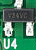
\includegraphics[width=.1\textwidth]{Component0}}
\caption{Template Component 0}
\label{fig:Component0}
\end{figure}

\begin{figure}[h]
\centerline{\includegraphics[width=.5\textwidth]{PCB}}
\caption{Source Image }
\label{fig:PCB}
\end{figure}

\begin{figure}[H]
\centerline{\includegraphics[width=.4\textwidth]{template_matching_ccoef_normed}}
\caption{Template Matching equation for a normalised correlation coefficient}
\label{fig:template_matching_ccoef_normed}
\end{figure}

When this code was run on the image, all of the components except \textit{Component 8} were found. This is the expected output for the PCB as this was the only component missing. This can be seen in Fig. \ref{fig:Missing_component_and_empty_place_on_PCB}.

If a component is found on the board it is outlined with a blue rectangle and the corresponding component number it outputted onto the terminal. When the code was run over multiple iterations, it reliably managed to identify that \textit{Component 8} was missing. 

In order to do a comprehensive test of the software, a picture of the board with the missing component added back on was used. Under these conditions, \textit{Component 8} was reliably and repeatably found in the correct location. This result shows that the template matching algorithm was in fact working on all the components and was not missing any on its run through. 

A flow chart for this task can be seen in Appendix \ref{appendix:task_3_flowchart}.

\begin{figure}
\centering
\subfigure[Missing Component Space on PCB]{
\includegraphics[width=.225\textwidth]{PCB_component_8}
}
\subfigure[Missing Component]{
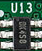
\includegraphics[width=.125\textwidth]{Component8}
}
\caption{Missing Component and Empty place on PCB}
\label{fig:Missing_component_and_empty_place_on_PCB}
\end{figure} 

\textit{A video of the code in operation can be seen in this \href{https://youtu.be/8uITJsA60Wk}{link}}

\subsection{Further Improvements}

Despite the Template Matching algorithm working, it is not robust. It will not work if there are differing orientations or scales. Fixing the scaling issues is relatively simple and can be done using template matching. To do multi-scaled template matching is simple. The template image is re-scaled and the template matching algorithm is run again. \cite{ref:open_cv_templae_matching_scaling} This approach is simplistic and can save a lot of effort in writing additional code and dealing with more fancy methods of template matching. 

Template matching is not a good solution if the template and source image are in different orientations. Instead another methods can be used such as Canny Edge Detection or Keypoint Detection. 

Canny Edge detection is one of the most popular edge detection algorithm developed by John F. Canny. It is a multi-stage process. It starts by utilising a Gaussian filter \cite{ref:Gaussian_filters} to reduce edge noise in the image. After this, the intensity gradient of the image is found using a Sobel kernel \cite{ref:sobel_kernal}. This then gets the first derivaive in both the x ($G_x$) and y ($G_y$) directions. The Edge Gradient is then calculated from this.  After this, Non-maximum suppression \cite{ref:non-maximum_supression} is used to remove any unwanted pixels that may not have made up the edge of the object. The final step is Hysteresis Thresholding \cite{ref:hysteresis_thresholding}. This stage is done to determine which edges are actually edges and which are not. 

Keypoint detection is used often to mark out the human body. It utilises a heatmap representation of each keypoint i.e. shoulders, hips, hands etc. \cite{ref:keypoint_detection} This type technique is often paired with a neural network to make the detection faster and more accurate. This kind of Keypoint Detection is very powerful and has many uses such as gesture recognition, sign languages understanding, and activity recognition along with many more. \cite{ref:keypoint_detection_using_deep_learning} Given the scope of this task, keypoint detection using a deep learning network would be deemed to be an over-engineered solution.

\subsection{Conclusion}

As per the two other examples, template matching worked well enough for the criteria provided. Despite this, template matching is rather limited and if anything more complex than a difference in scaling, this approach would prove to be ineffective. A more robust and comprehensive solution would be required in the real world.

A combination of the three previous example of cross correlation could provide a lightweight initial set of tests backed up by a more computationally intensive but more robust solution. This could be used to evaluate more complex matching tasks, initially running the more lightweight, but less powerful algorithms before moving towards heavyweight but more thorough methods afterwards. 


\bibliographystyle{IEEEtran}
\bibliography{refs}

The code can be found on GitHub \href{https://github.com/LukeDWaller99/Aint308}{here!} 

\onecolumn

\begin{appendix}

\subsection{Flowchart for Task 1}

\begin{figure}[H]
\centerline{\includegraphics[width=\textwidth]{task_1_flowchart}}
\end{figure}

\label{appendix:task_1_flowchart}

\subsection{Pendulum in the RGB and HSV Colour Space}

\begin{figure}[H]
\centering
\subfigure[Pendulum in the RGB Colour Space]{
\includegraphics[width=.5\textwidth]{pendulum_rgb_space}
}
\subfigure[Pendulum in the HSV Colour Space]{
\includegraphics[width=.5\textwidth]{pendulum_hsv_space}
}
\end{figure}

\label{appendix:pendulum_rgb_hsv_space}

\subsection{Isolated Rectangle at the End of the Pendulum}

\begin{figure}[H]
\centerline{\includegraphics[width=.5\textwidth]{pendulum_isolate_colours}}
\end{figure}

\label{appendix:isolated_rectangle}

\subsection{Full Size Graph of Pendulum Angle Against Time}

\begin{figure}[H]
\centerline{\includegraphics[width=1.2 \textwidth, angle = 90]{angle_output}}
\end{figure}

\label{appendix:angle_output_full_size}

\subsection{Full Code - Task 2 }

\begin{figure}[H]
\centerline{\includegraphics[width=.6\textwidth]{CW1_Task_2_full_code}}
\end{figure}

\label{appendix:task_2_full_code}

\subsection{Flowchart for Task 2}

\begin{figure}[H]
\centerline{\includegraphics[width=0.6\textwidth]{task_2_flowchart}}
\end{figure}

\label{appendix:task_2_flowchart}

\subsection{Template Matching Components}

\begin{figure}[H]
\centering
\subfigure[Component 0]{
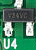
\includegraphics[width=.2\textwidth]{Component0}
}
\subfigure[Component 1]{

\includegraphics[width=.2\textwidth]{Component1}
}
\subfigure[Component 2]{
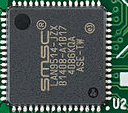
\includegraphics[width=.2\textwidth]{Component2}
}
\subfigure[Component 3]{
\includegraphics[width=.2\textwidth]{Component3}
}
\subfigure[Component 4]{
\includegraphics[width=.2\textwidth]{Component4}
}
\subfigure[Component 5]{
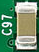
\includegraphics[width=.2\textwidth]{Component5}
}
\subfigure[Component 6]{

\includegraphics[width=.2\textwidth]{Component6}
}
\subfigure[Component 7]{
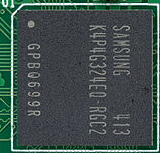
\includegraphics[width=.2\textwidth]{Component7}
}
\subfigure[Component 8]{
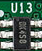
\includegraphics[width=.2\textwidth]{Component8}
}
\subfigure[Component 9]{
\includegraphics[width=.1\textwidth]{Component9}
}
\end{figure}

\label{appendix:template_matching_components}

\subsection{Flowchart for Task 3}

\begin{figure}[H]
\centerline{\includegraphics[width=\textwidth]{task_3_flowchart}}
\end{figure}

\label{appendix:task_3_flowchart}


\end{appendix}

\end{document}
